% --- REAL-WORLD APPLICATIONS --- %
\newpage
\section{Real-world applications}
\label{sec:applications}

Lambert's problem solvers have lots of applications because they retrieve the
solution to the \textit{boundary value problem} (BVP) of the restricted two-body
dynamics problem.  This solution is nothing but the conic trajectory which the
body will follow as time evolves. The previous fact makes Lambert's problem to be
usually included within the initial \textit{orbit determination topic} (IOD).

However, the most common applications for the Lambert's problem are targeting,
maneuvering and rendezvous ones. For example, if it is desired to navigate from
an initial position to a final one over a finite amount of time then, the orbit
which must be followed is the one obtained by solving the Lambert's problem.

In fact, Lambert's solvers routines were implemented in the \textit{Apollo
  Guidance Computer} (AGC\footnote{The original source code for the AGC has been
  published under a Public Domain license in
  https://github.com/chrislgarry/Apollo-11}) for the calculation of transfer
trajectories and reentry ones. In the \citetitle{apollo1972}, it is claimed that
the algorithms (AGC programs P-31 to P-37) took between 15 to 30 minutes to
compute a solution, which showed the necessity of having better performance
solvers for future missions.

% Example of Apollo Lunar Module rendezvous %
\vspace{0.5cm}
\begin{figure}[h]
  \centering
  \includegraphics[scale=1]{apollo_trajectory.png}
  \caption{After the \textit{Lunar Module} (LM) was launched into a
    \textit{Constant Delta Height} (CDH) orbit, a set of targetting
    maneuvers were required to perform a rendezvous with the \textit{Command
      and Service Module} (CSM). The AGC made use of its own Lambert's
    solvers routines to calculate the required impulses in order to correct
    the course of the LM spacecraft.}
  \label{fig:apollo_trajectory}
\end{figure}

Course corrections, as shown in figure \ref{fig:apollo_trajectory}, might be
required during the transfer, forcing to compute a new solutions by calling the
different transfer routines several times in order to reach final aiming
location.

Last application is closely related with the mission analysis field. Solving
Lambert's problem for a given set of launching and arrival dates leads to a
collection of particular orbits, each one corresponding to a transfer arc.
Those conic trajectories show a different characteristic velocity, directly
related with the amount of required energy.  Contour maps representing this set
of solutions are known as porkchop plots and it is possible to observe that minimum
transfer points exist within these figures.  These locations in the contour
figure are usually selected for space missions launch and arrival dates.

% Figure showing optimal transfer for Mars perseverance
\begin{figure}[h]
  \centering
  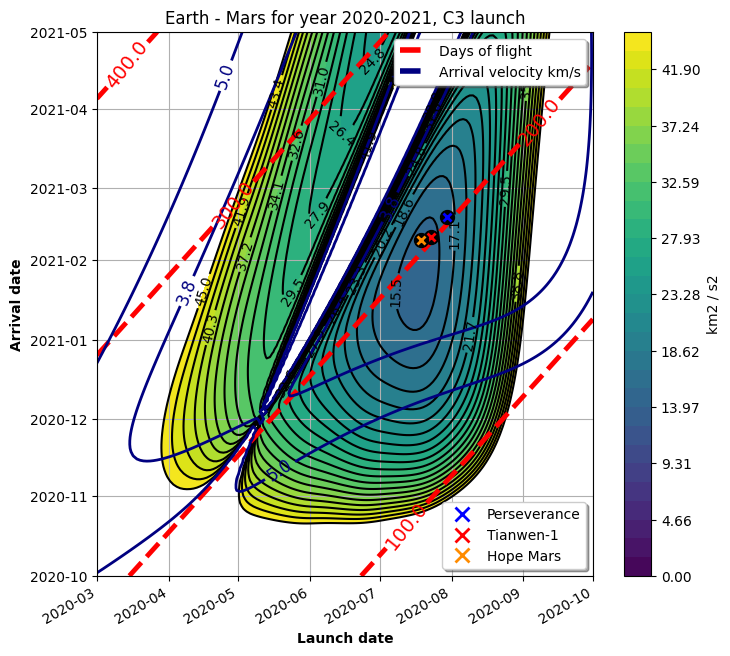
\includegraphics[width=\linewidth]{static/porkchop.png}
  \caption{Porkchop for Earth-Mars transfer arrival energy for years 2020-2021.
    Each point in the figure is obtained by solving the Lambert's problem in order
    to compute departure $C_{3}$ (characteristic energy). Notice the optimal
    transfer dates are being used by latest missions about this planet: Perseverance,
    Tianwen-1 and Hope Mars.}
  \label{fig:porkchop_perseverance}
\end{figure}

With all previous examples on mind, it is clear that Lambert's applications
require from high performance solving routines to compute in a fast and reliable
way final desired orbit trajectories.
